\documentclass{beamer}
\usepackage{amsmath}
\usepackage{amssymb}
\usepackage{graphicx}
\begin{document}
\title{Nonlinear Analysis of VR Synchrony}
\author{Howon Lee}
\maketitle

\begin{frame}
  \frametitle{Introduction}
  Social Synchrony, previous results
\end{frame}
\begin{frame}
  \frametitle{Questions}
  Does nonlinearity matter?
\end{frame}
\begin{frame}
  \frametitle{Data Description}
  Data: AS Won creativity study, Kinect data

  Ad hoc differencing of Kinect data
\end{frame}
\begin{frame}
  \frametitle{Mutual Information}
  Intuition, formalism

  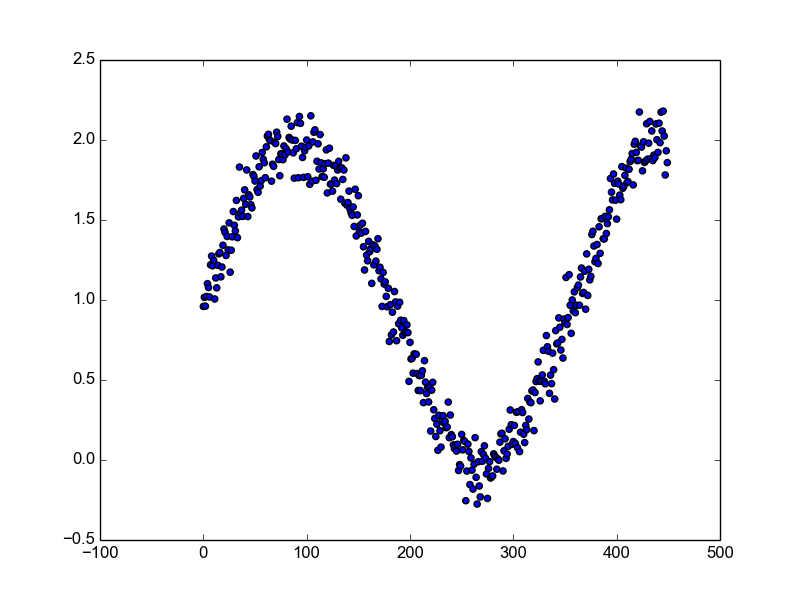
\includegraphics[scale=0.2]{mi_ex}
  
  $$I(x,y) = \sum_{x,y}P(x,y) \ln \frac{P(x,y)}{P(x)P(y)}$$

  How to discretize?
\end{frame}
\begin{frame}
  \frametitle{Analytic Signal Methods}
  Hilbert transform representation, phase not amplitude.

  Phase Synchrony Index : $\gamma = |<e^{i(n\phi_x - m\phi_y)}>|$
\end{frame}
\begin{frame}
  \frametitle{Graph-Based Methods}
  Many ones exist: recurrence matrix, visibility graph, etc etc etc

  Reversability: turning this into a transform

  Stack graph
\end{frame}
\begin{frame}
  \frametitle{Results}
  Go see results
\end{frame}
\begin{frame}
  \frametitle{Thanks}
  Jeremy N Bailenson
  Andrea S Won
  VHIL
  Surya Ganguli
\end{frame}
\begin{frame}
  Questions?
\end{frame}
\end{document}

